コンテンツ提供機能は,教材提供者が情報倫理に関するコンテンツを提供するための機能である.
本機能ではWeb上で教材提供者のみがコンテンツの投稿と管理ができる.
コンテンツを投稿する際に必要な情報は,コンテンツのタイトルと本文である.
本文はマークダウン形式で記入可能であり,画像や動画の挿入が容易にできる.またプレビュー機能もあるため投稿する前にどのような見た目で投稿されるのかを確認できる.
コンテンツを投稿する際のGUIは図\ref{teikyou}の通りである.

また,教材提供者はコンテンツを管理するためのグループに参加する.
そのグループはすべてのコンテンツに対して公開または非公開を選択することでコンテンツを管理する.
グループに参加している教材提供者全員が認可したコンテンツのみが学習者に公開される.
これにより,コンテンツの正当性を担保できる.
教材提供者をグループに参加させるには,図\ref{group_register}のようにして教材提供者のアカウントを選択し教材提供者のグループに登録する.

\begin{figure}[htbp]
    \begin{center}
        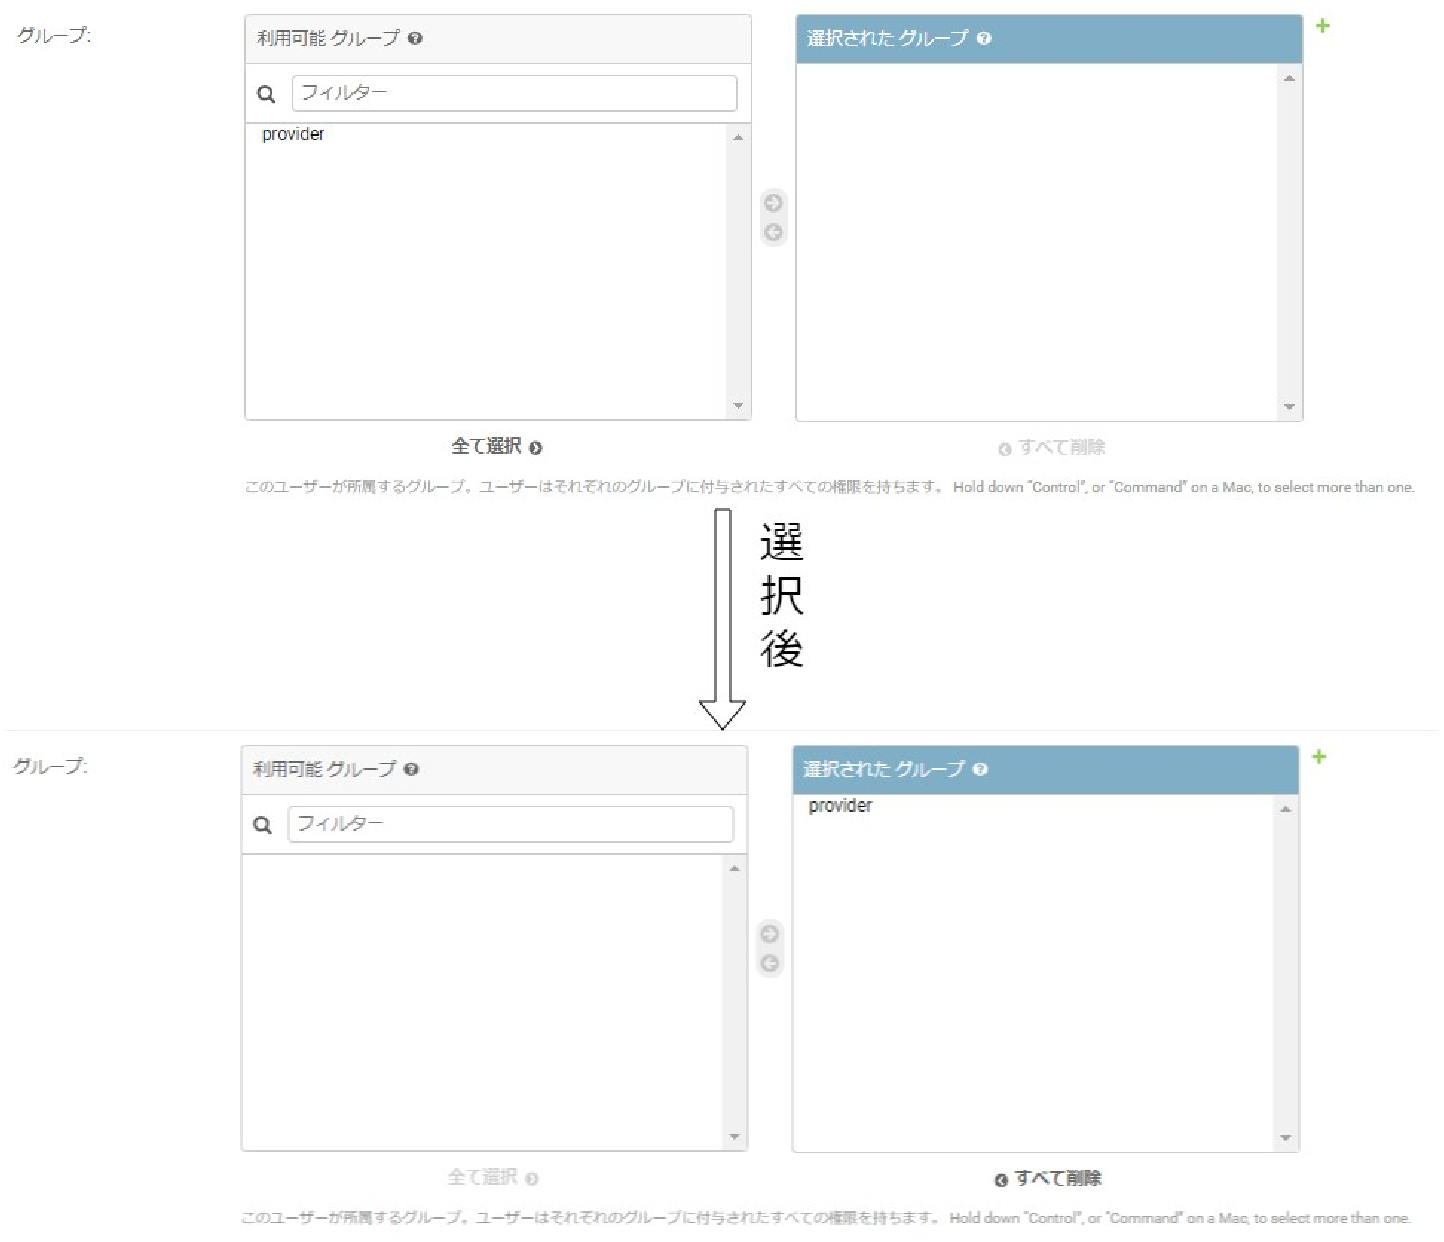
\includegraphics[width=13cm,height=12cm,keepaspectratio]{group_register-crop.pdf}\\
        %includegraphicsの詳しい使い方ははLaTeXの参考書を参照.
    \end{center}
    \caption{グループ登録のGUI}
    \label{group_register}
\end{figure}